\documentclass[11pt, a4paper]{article}

\usepackage[T1]{fontenc}
\usepackage[utf8]{inputenc}
\usepackage[norsk]{babel}
\usepackage{amsmath}
\usepackage{amsfonts}
\usepackage{amssymb}
\usepackage{graphicx}
\usepackage{verbatim}
\usepackage{caption}
\usepackage{subcaption}
\usepackage{subfig}
\usepackage{float}
\usepackage{program}
\usepackage{commath}


\begin{document}
\begin{titlepage}

  \title{\normalsize FYS3150 Computational Physics 2014\\
  \vspace{10mm}
  \huge Oblig 2\\
  \vspace{10mm}
  \normalsize {\bf Løysning av Schrödinger likninga for to elektron i ein tredimensjonal oscillator brønn.}}

  \author{Øyvind Sigmundson Schøyen}

\end{titlepage}

\maketitle

\newpage
\begin{abstract}
  Me har sett på Schrödinger likninga for å finne potensialet til to elektron i ein harmonisk oscillator brønn. Oppgåven har stort sett gått ut på å løyse 
  eit eigenverdi og eigenvektor problem for ein andreordens differensiallikning. Me har nytta Jacobirotasjon til å finne eigenverdiane og eigenvektorane. 
  Desse har me brukt til å plotte bølgjefunksjonen mot avstanden $\rho$. Me har sett på skjelnaden i potensialet for to elektron med og uten Coulomb interaksjon for 
  forskjellige frekvensar. Me har kun sett på bølgjefunksjonen for grunntilstanden og dei to fyrste eksiterte tilstandane. Til slutt har me ei feilanalyse over eigenverdiane 
  me får frå Jacobi. All kjeldekode ligg på github. \\ \\
  God lesning! \\ \\
  \texttt{https://github.com/Schoyen/FYS3150/tree/master/Oblig2}
\end{abstract}

\newpage
  \tableofcontents
\newpage

\section{Introduksjon}
  I dette prosjektet er me interesserte i å løyse Schrödinger likninga for to elektron. Likninga er skrive om slik at me kan jobbe med eit eit-lekam problem.
  Me nyttar lineær algebra for å løyse differensiallikningane som eit sett med lineære likningar. Måten me gjer dette på er ved Jacobirotasjon 
  for å finne eigenvektorar og eigenverdiar. Til slutt vil me plotte bølgjefunksjonen for grunntilstanden til elektrona ved hjelp av eigenvektorane og 
  eigenverdiane.


\section{Jacobirotasjon}
  For å løyse eigenverdi- og eigenvektorproblema vil me nytte Jacobirotasjon. Dette er ein algoritme som, etter ein rekke similaritetsformasjonar, vil 
  gjere alle ikkje-diagonale matriseelement til null. Denne algoritmen er likevel ikkje ein veldig effektiv algoritme då me ved ein rotasjon kan kome 
  i skade for å gjere eit element som tidligare var null til å bli ikkje-null. Numerisk kan det og ta lang tid før elementa vert null. Me vil difor heile 
  tida teste verdiane mot ein toleranse for å sjå om dei er nære nok null.

\subsection{Algoritma}
    Ein similaritetstransformasjon er gitt ved 
    \begin{align*}
      B = S^TAS
    \end{align*}
    kor $S$ er ein ortogonal matrise der $SS^T = SS^{-1} = I$. Matrisa $S$ transformerer $A$ ein vinkel $\theta$ i planet medan $S^T$ tek ho tilbake.
    Me vil då velje $\theta$ slik at alle ikkje-diagonale element vert null. Når me gjer dette numerisk må me gjere ein rekke similaritetstransformasjonar 
    for å oppnå dette. Då har me
    \begin{align*}
      B = S_n^T \dots S_1^TAS_1 \dots S_n.
    \end{align*}
    Kvar matrise $S$ og $S^T$ er identitetsmatrisa med unntak av elementa $s_{kk} = s_{ll} = \cos{\theta}$, $s_{kl} = -s_{lk} = -\sin{\theta}$ og 
    $s_{ii} = 1$ for $i \ne k$ og $i \ne l$. Produktet $B = S^TAS$ kan då skrivast som
    \begin{align*}
      b_{ii} &= a_{ii}, \qquad i \ne k, \ i \ne l \\
      b_{ik} &= a_{ik}\cos{\theta} - a_{il}\sin{\theta}, \qquad i \ne k, \ i \ne l \\
      b_{il} &= a_{il}\cos{\theta} + a_{ik}\sin{\theta}, \qquad i \ne k, \ i \ne l \\
      b_{kk} &= a_{kk}\cos^2{\theta} - 2a_{kl}\cos{\theta}\sin{\theta} + a_{ll}\sin^2{\theta} \\
      b_{ll} &= a_{ll}\cos^2{\theta} + 2a_{kl}\cos{\theta}\sin{\theta} + a_{kk}\sin^2{\theta} \\
      b_{kl} &= (a_{kk} - a_{ll})\cos{\theta}\sin{\theta} + a_{kl}(\cos^2{\theta} - \sin^2{\theta}).
    \end{align*}
    Me vil no velje $\theta$ slik at alle ikkje-diagonale element $b_{kl}$ i praksis vert null. For kvar iterasjon bør me i teorien teste om alle
    dei ikkje-diagonale elementa er mindre enn ein toleranse $\epsilon$. Me vil derimot ikkje gjer dette då det er ein tidkrevande prosess. 
    Erstatninga vert då å sjå om det største elementet blant dei ikkje-diagonale elementa er mindre enn $\epsilon$. Dette vil då vere
    \begin{align*}
      \abs{a_{kl}} = \text{max}_{i \ne j}\abs{a_{ij}}.
    \end{align*}
    Me krever at $b_{kl} = b_{lk} = 0$. Det gjer oss likninga
    \begin{align}
      a_{kl}(c^2 - s^2) + (a_{kk} - a_{ll})cs = b_{kl} = 0.
    \end{align}
    Me definerer no 
    \begin{align*}
      \tau = \frac{a_{ll} - a_{kk}}{2a_{kl}} \qquad \Rightarrow \qquad a_{ll} - a_{kk} = 2\tau a_{kl}.
    \end{align*}
    Setter dette inn i (1) og får
    \begin{align*}
      &a_{kl}c^2 - a_{kl}s^2 - 2\tau a_{kl}cs = 0, \\
      \Rightarrow \qquad &a_{kl} - a_{kl}\frac{s^2}{c^2} - 2\tau a_{kl}\frac{s}{c} = 0. \\
    \end{align*}
    Siden $c = \cos{\theta}$ og $s = \sin{\theta}$ vil me få 
    \begin{align*}
      &a_{kl} - a_{kl}\tan^2{\theta} - 2\tau a_{kl} \tan{\theta} = 0, \\
      \Rightarrow \qquad &1 - t^2 - 2\tau t = 0, \\
      \Rightarrow \qquad &t^2 + 2\tau t - 1 = 0,
    \end{align*}
    kor $t = \tan{\theta}$. Me vil då få 
    \begin{align*}
      t &= \frac{-2\tau \pm \sqrt{4\tau^2 - 4(-1)}}{2} \\
      &= -\tau \pm \sqrt{1 + \tau^2}.
    \end{align*}
    For å unngå avrungdingsfeil ved $\tau >> 0$ gonger me andregradslikninga med den konjugerte. Det vil gje oss
    \begin{align*}
      t &= \left( -\tau \pm \sqrt{1 + \tau^2} \right)\left( \frac{\tau \pm \sqrt{1 + \tau^2}}{\tau \pm \sqrt{1 + \tau^2}} \right) \\
      &= \frac{-\tau^2 + (1 + \tau^2)}{\tau \pm \sqrt{1 + \tau^2}} = \frac{1}{\tau \pm \sqrt{1 + \tau^2}},
    \end{align*}
    som gjer oss
    \begin{align*}
      t = \frac{1}{\tau \pm \sqrt{1 + \tau^2}} \qquad \lor \qquad t = \frac{1}{\tau - \sqrt{1 + \tau^2}}.
    \end{align*}
    Me vil no velje den minste av røttene $t$ slik at $c$ og $s$ henholdsvis går mot ein og null ved
    \begin{align*}
      c = \frac{1}{\sqrt{1 + t^2}}, \qquad s = tc.
    \end{align*}
    Det gjer me ved å teste verdien av $\tau$. For $\tau > 0$ vil me velje 
    \begin{align*}
      t = \frac{1}{\tau + \sqrt{1 + \tau^2}}.
    \end{align*}
    For $\tau \leq 0$ vil me velje
    \begin{align*}
      t = \frac{1}{\tau - \sqrt{1 + \tau^2}}.
    \end{align*}
    Då vil me kunne begrense vinkelen $\theta \leq \frac{\pi}{4}$ slik at differansen mellom matrisa $B$ og $A$ vert så liten som mogleg ved formelen
    \begin{align*}
      \lvert\lvert B - A \rvert\rvert_F^2 = 4\underbrace{(1 - c)}_{= 0 \text{ for } c \to 1}\sum_{i = 1, i\ne k, l}^n(a_{ik}^2 + a_{il}^2) + \frac{2a_{kl}^2}{c^2}.
    \end{align*}
    Me vil fortsette desse operasjonane heilt til $\text{max}(a_{ij})^2 \leq \epsilon$ for $i \ne j$.

  \subsection{Implementering}
    Algoritma vert implementert i ein klasse med tre metodar som løyser eigenverdi og eigenvektor problemet. Denne implementasjonen er kommentert i programmet.



\section{Resultat}
  Denne seksjonen vil bli delt opp i tre deler. Me vil diskutere metoden i seg sjølv kor me ser på køyretid og stabilitet. % Big O, Jacobi mot 
  % Armadillo og storleik på matrise.
  Me vil sjå på energinivåa til elektrona med, og uten, Coulomb interaksjon for forskjellige $\omega_r$ og $\rho_{\text{max}}$. Eg har valt å gjere dette 
  ved Jacobi. Dette krev at me normaliserer eigenvektorane for å få riktige verdiar. Det vil bli forklart i meir nøyaktighet. % FORKLAR!
  Til slutt har eg lagt ved ein feilanalyse på eigenverdiane som funksjon av $n_{\text{step}}$.

  \subsection{Jacobi}
    Jacobirotasjon er ein reknetung algoritme. Denne metoda bryt veldig kjapt ned når ein lager ei stor matrise. For vårt formål er det difor 
    essensielt at me uttnyttar peikar- og referansemoglegheitane i C++ for å unngå unødvendig tidbruk på lagring. Køyretida til metoden går som $\mathcal{O}(n^3)$ for rotasjon. 
    Mykje av grunnen til at metoda er treig kjem frå det faktum at me står i fare for å gjere eit element som er null til ikkje-null ved ein rotasjon. Me merker fort når matrisa 
    blir stor at tidbruken stig veldig kjapt. Ein samanlikning av $\texttt{eig\_sym}$ frå Armadillo og Jacobi gjer oss køyretidene i sekund i tabellen under.
    \begin{center}
      \begin{tabular}{|l||l|l|l|}
        \hline
        Steg & \text{Armadillo} & \text{Jacobi} & Antal iterasjonar \\
        \hline
        \input{koyretid.txt} \\
        \hline
      \end{tabular}
    \end{center}
    Me ser korleis Armadillo aukar jamnt med $n$-verdiane medan Jacobi stig eksponensielt. Med ei kubisk køyretid vil me veldig kjapt nå eit tak over kor stor matrisa vår kan 
    vere. I programmet vårt set me ei begrensning for kor mange iterasjonar me tillet. Når matrisa vert stor nok vil denne begrensninga ikkje lengre tjene formålet då ho vil 
    verte for stor for våre praktiske formål. Ei senkning av denne kan igjen føre til eit for lite antal iterasjoner og gå på bekostning av presisjon. Antal iterasjonar som
    står oppførte er det antalet det tek før alle ikkje-diagonale matriseelement i praksis er null. Metoden i seg sjølv 
    er difor stabil for mindre matrisar, men kan fort bli ubrukeleg for større matrisar. Fordelane med metoda er at ho er enkel å implementere og er effektiv ved 
    parallellprogrammering. Me kjem diverre ikkje inn på dette i denne oppgåva. \\

  \subsection{Potensialenergien til elektron med og uten Coulomb interaksjon}
    I dette prosjektet har me rekna på potensialenergien til to elektron i ein oscillator brønn. Fyrst har me sett på eit døme uten Coulomb interaksjon. Då har me definert 
    det harmoniske oscillator potensialet ved $V_i = \rho_i^2$. For dette dømet har me eksakte løysningar på eigenverdiane me får frå Jacobi. Dette avheng derimot av val 
    av $n_{\text{step}}$ og $\rho_{\text{max}}$. For å få eit svar med fire siffers nøyaktighet må me inngå nokre kompromiss for $\rho_{\text{max}}$. Dette kjem me tilbake 
    til i feilanalysa. Når me ser på potensialenergien med Coulomb interaksjon vil me få eit potensial gitt ved $V_i = \omega_r^2\rho^2 + \frac{1}{\rho}$. Her vil me fortsatt vere 
    avhengige av $n_{\text{step}}$ og $\rho_{\text{max}}$, men me vil no i tillegg ha ein avhengighet til $\omega_r$. Valet av $\rho_{\text{max}}$ vil vere direkte knytta til 
    $\omega_r$. Me nyttar artikkelen til M. Taut slik at me kan finne verdiar med ein eksakt løysning. Diverre vil kun nokre få av desse løysningane vere relevante for vårt formål. i
    \\ \\
    Me er interesserte i $\omega_r = 0.01$, $\omega_r = 0.5$, $\omega_r = 1$ og $\omega_r = 5$. Artikkelen til M. Taut hjelper oss med to av desse. Me kan finne ei eksakt løysning 
    for $\omega_r = 0.05$ og $\omega_r = 0.25$. Me finn då ein $\rho_{\text{max}}$ som gjer oss eksakte svar. Me tolkar difor at for $\omega_r = 0.01$ og $\omega_r = 0.5$ så vert det 
    tilnærma likt. Me kjem då fram til at frekvensane $\omega_r = 0.01$ og $\omega_r = 0.5$ vil gje oss $\rho_{\text{max}} \approx 50$ og $\rho_{\text{max}} \approx 10$. Desse 
    frekvensane tilsvarer svak Coulomb interaksjon og me vil få ``flate kurver''. For $\omega_r = 1$ vil me velje same $\rho_{\text{max}}$ som for det tidlegare potensialet. 
    Me vil då sjå at leddet $\frac{1}{\rho}$ utgjer ein forskyvning av bølgjefunksjonen. Det gjer oss $\rho_{\text{max}} = 5$. For den siste frekvensen $\omega_r = 5$ vil me ha ein 
    liten $\rho_{\text{max}}$ då dette utgjer ein sterk Coulomb interaksjon. Bølgjefunksjonen vil då bli bratt og kort. Me vel $\rho_{\text{max}} = 2$. % Tolkning
    \\
    Siden me behandlar alle verdiar som dimensjonslause er me interesserte i å plotte normaliserte eigenvektorar. Det gjer me ved formelen
    \begin{align*}
      \mathbf{v} = \frac{\mathbf{v}}{\sqrt{\int_{\rho_0}^{\rho_{\text{max}}}{v^2 \ d\rho}}}.
    \end{align*}
    Numerisk nyttar me trapesregelen for å rekne ut integralet. Alle grafane vil difor kun spenne ut eit areal på 1. \\ \\
    Alle plott er plotta for $n_{\text{step}} = 200$.

    \subsubsection{Plott for $\omega_r = 0.01$.} 
      Sjølv om den eksakte løysninga for $\omega_r = 0.05$ vil gje oss ein $\rho_{\text{max}} \approx 50$ vil me for $\omega_r = 0.01$ ha ein $\rho_{\text{max}}$ som er mykje større.  
      For å få eit plott som ikkje blir ``trykt'' ned mot slutten på grunn av randkrava har eg plotta for $\rho_{\text{max}} = 300$ i tillegg. Diverre resulterer dette i eit lite 
      informativt plott når me plottar for alle frekvensane i lag.
      \begin{figure}[H]
        \centering
        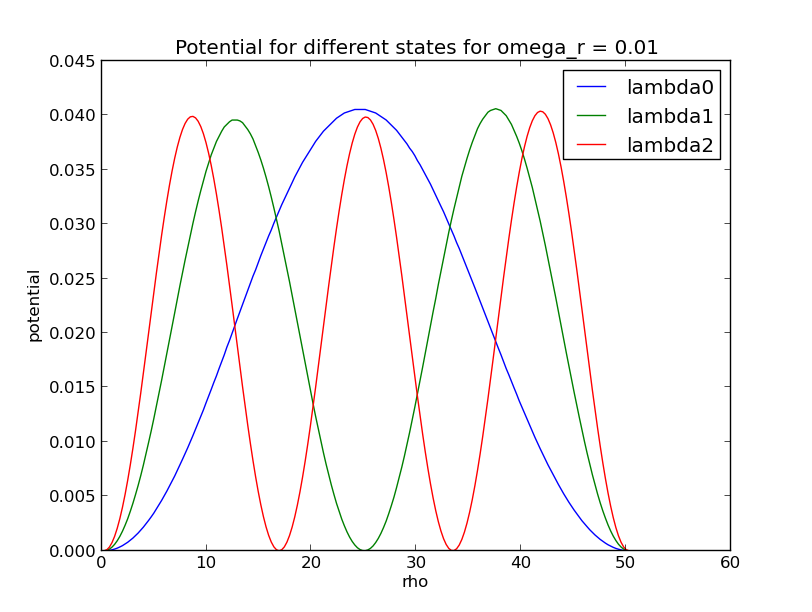
\includegraphics[width=300px]{omega001kort.png}
        \caption{Her har me plotta for $\rho_{\text{max}} = 50$. Me ser korleis kurva vert avkappa mot slutten grunna randkrava.}
      \end{figure}
      \begin{figure}[H]
        \centering
        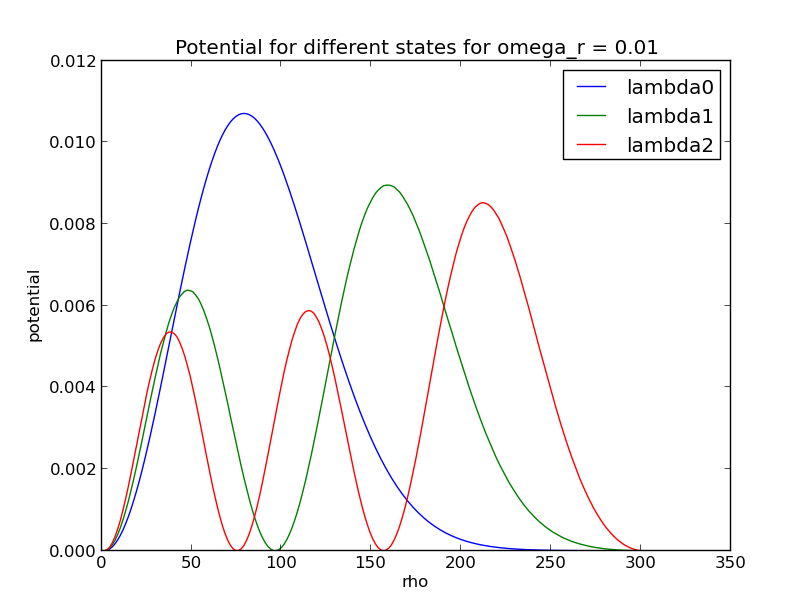
\includegraphics[width=300px]{omega001lang.png}
        \caption{Her har me plotta for $\rho_{\text{max}} = 300$. I dette dømet vil ikkje kurva vere begrensa av randkrava. Me kan sjå på verdiane til potensialet at kurva vil vere 
        mykje mindre enn dei for kortare $\rho_{\text{max}}$. Dette då arealet under alle grafane vil vere 1.}
      \end{figure}

    \subsubsection{Plott for $\omega_r = 0.5$.}
      Her vil me ha ei tilnærma løysning frå artikkelen til M. Taut. 
      \begin{figure}[H]
        \centering
        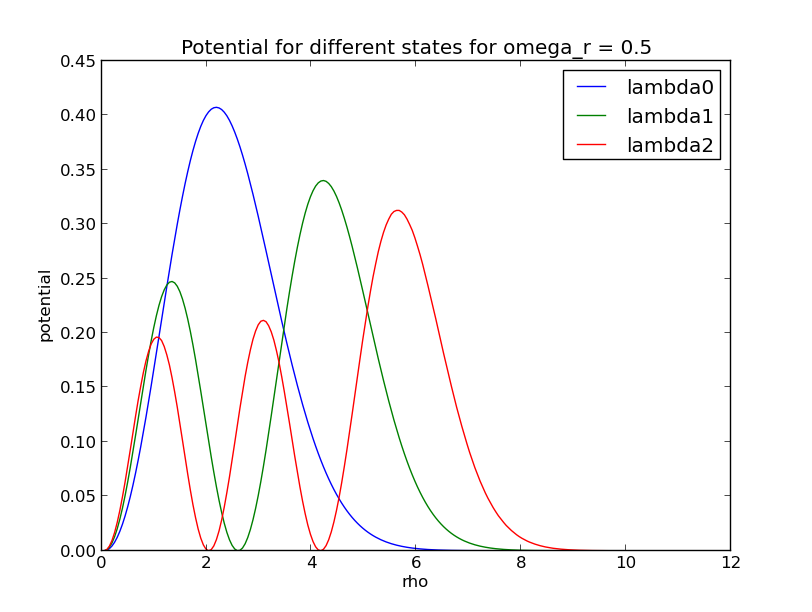
\includegraphics[width=300px]{omega05.png}
        \caption{Plott for $\rho_{\text{max}} = 10$. Me ser at kurva ikkje vert kappa av frå randkrava. Legg merke med aukninga i potensialet. Arealet vil fortsatt vere 1, men 
        siden $\rho_{\text{max}}$ er mykje mindre enn for det forrige plottet vil verdien stige.}
      \end{figure}

    \subsubsection{Plott for $\omega_r = 1$.}
      I dette plottet vil det vere hensiktsmessig å ha med samanlikning av det føregåande og nåværande potensialet. Dette då me vil kunne sjå ei forskyvning. Viss me auker 
      $\frac{C}{\rho}$-leddet i potensialet med Coulomb interaksjon vil me kunne sjå ei tydeleg forskyvning.
      \begin{figure}[H]
        \centering
        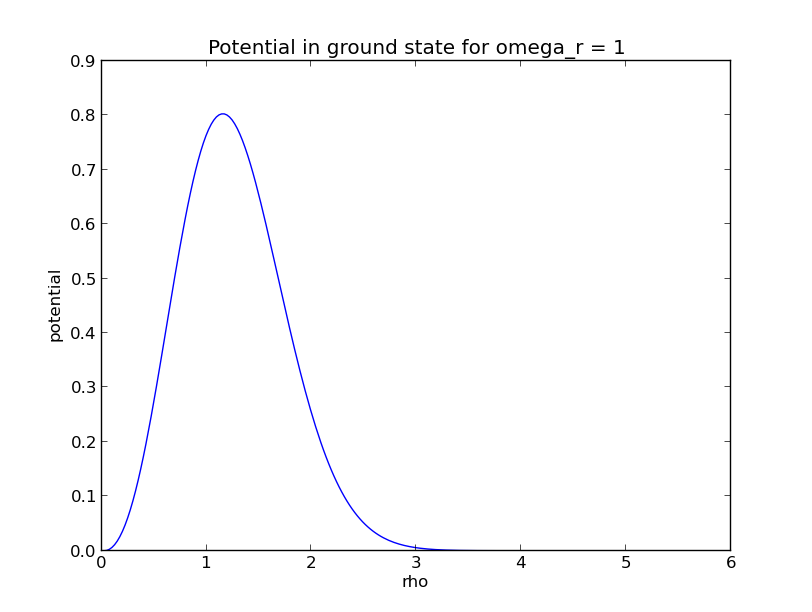
\includegraphics[width=300px]{omega1.png}
        \caption{Plott for $\rho_{\text{max}} = 5$.}
      \end{figure}
      \begin{figure}[H]
        \centering
        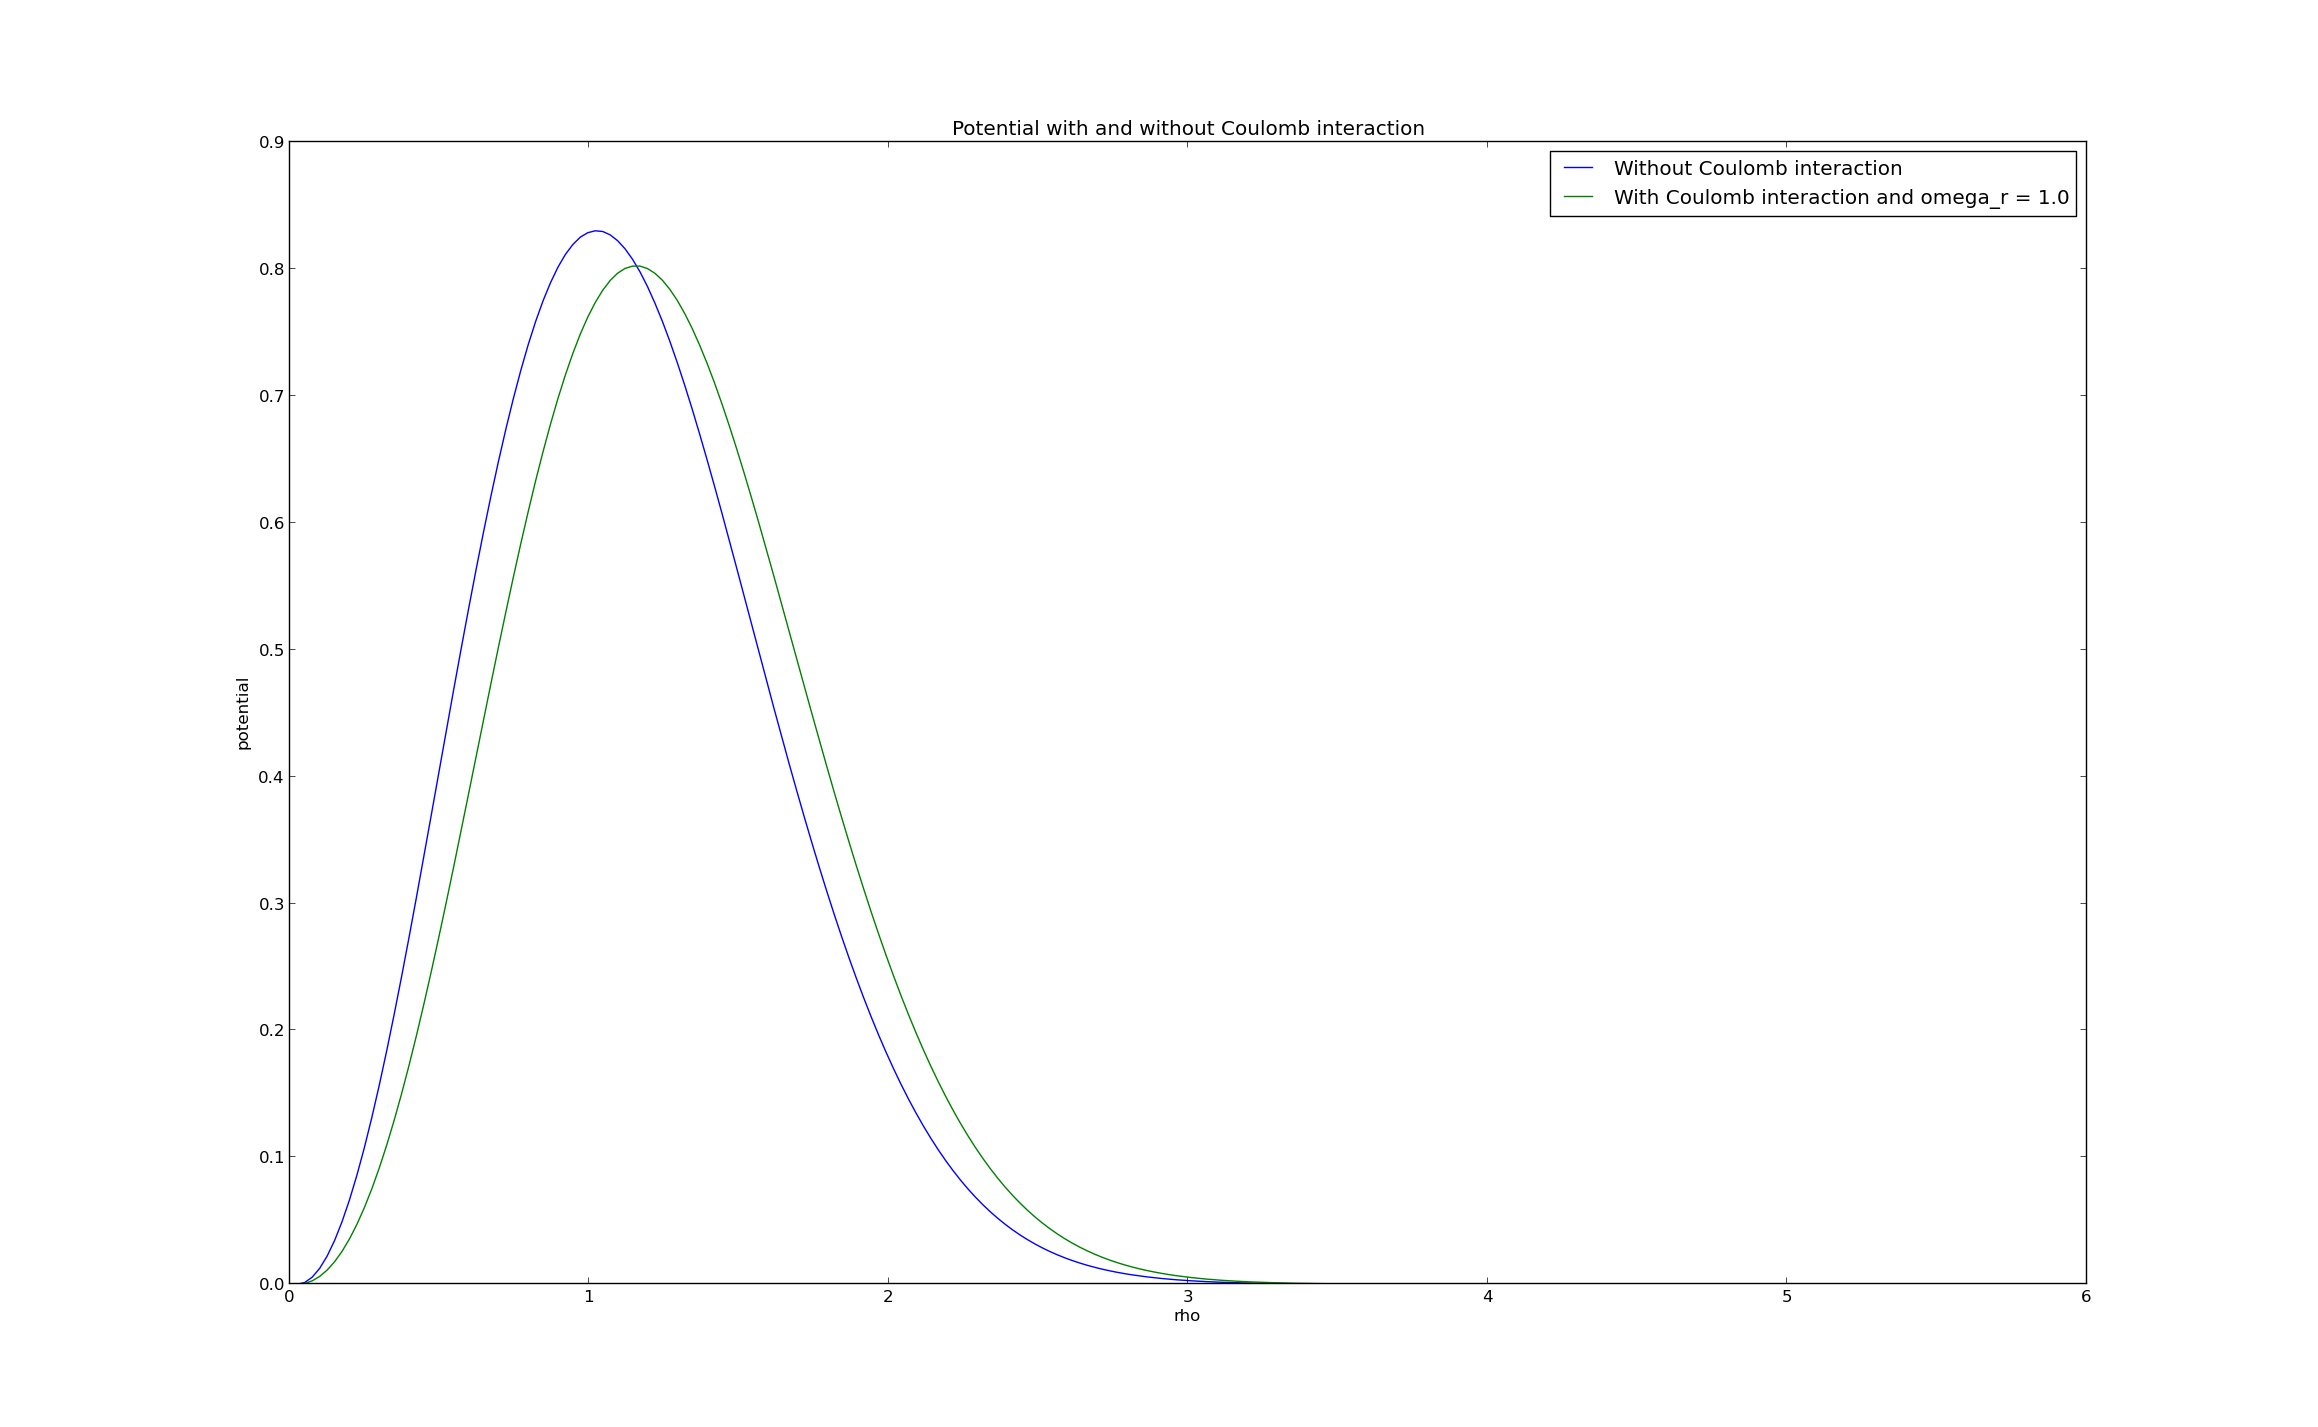
\includegraphics[width=400px]{omega1to.png}
        \caption{Her er $V_i = \omega_r^2\rho^2 + \frac{1}{\rho}$ for den grøne grafen.}
      \end{figure}
      \begin{figure}[H]
        \centering
        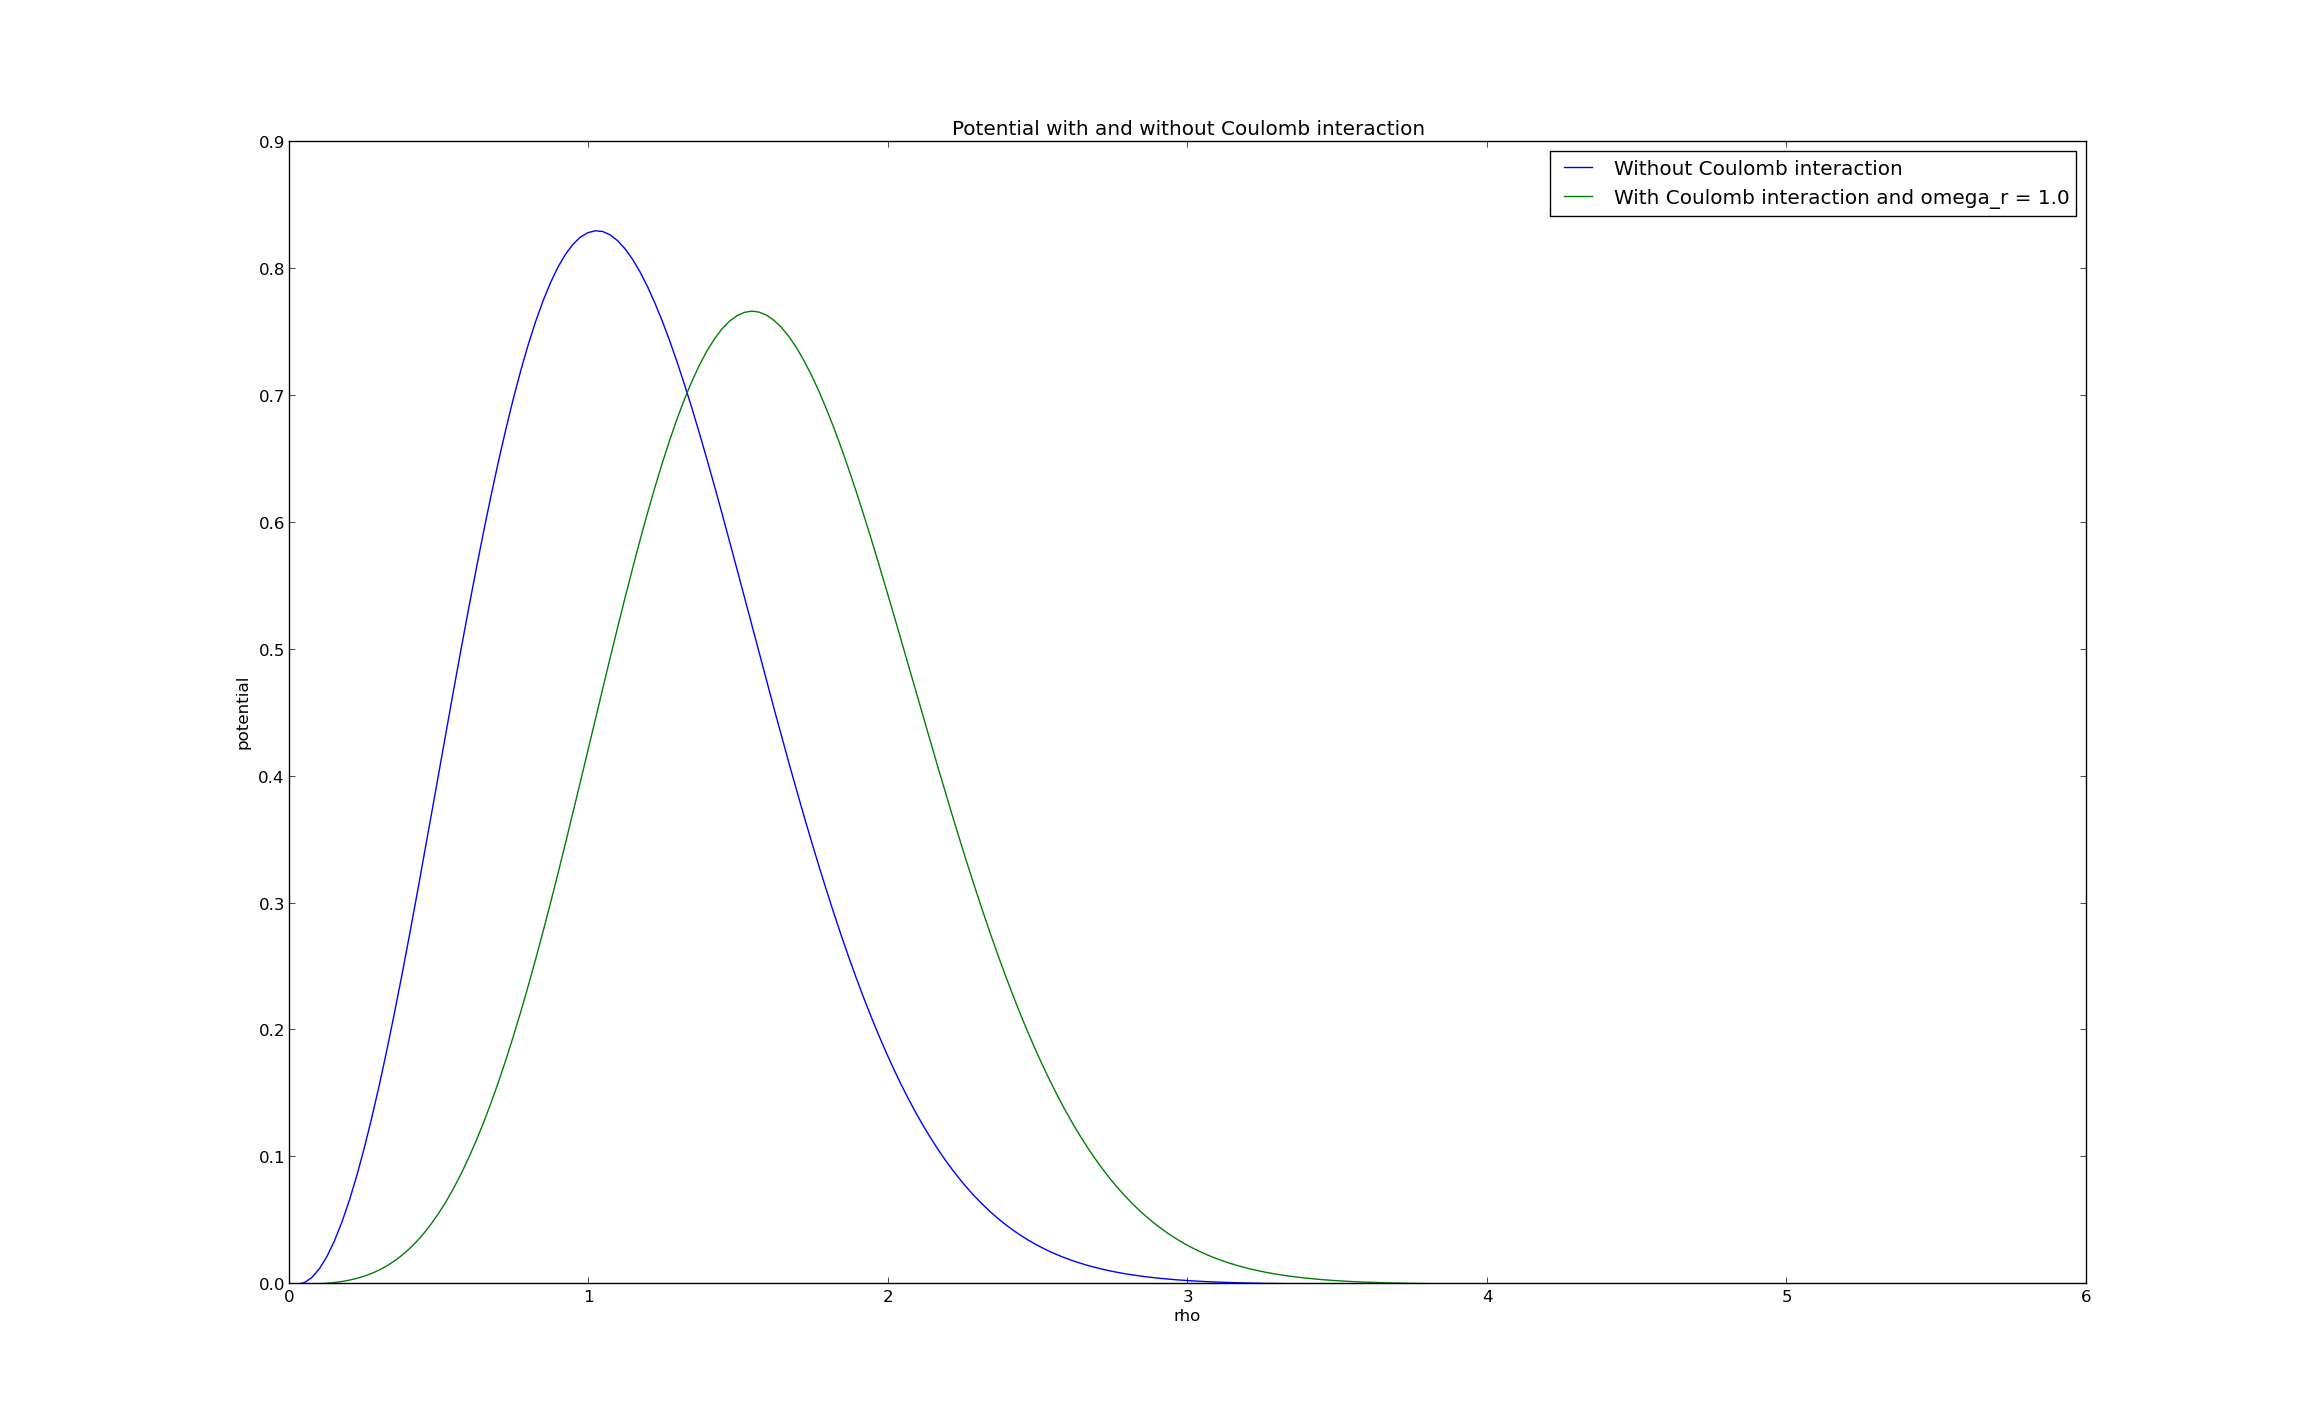
\includegraphics[width=400px]{omega1to5.png}
        \caption{Her er $V_i = \omega_r^2\rho^2 + \frac{5}{\rho}$ for den grøne grafen.}
      \end{figure}
      \begin{figure}[H]
        \centering
        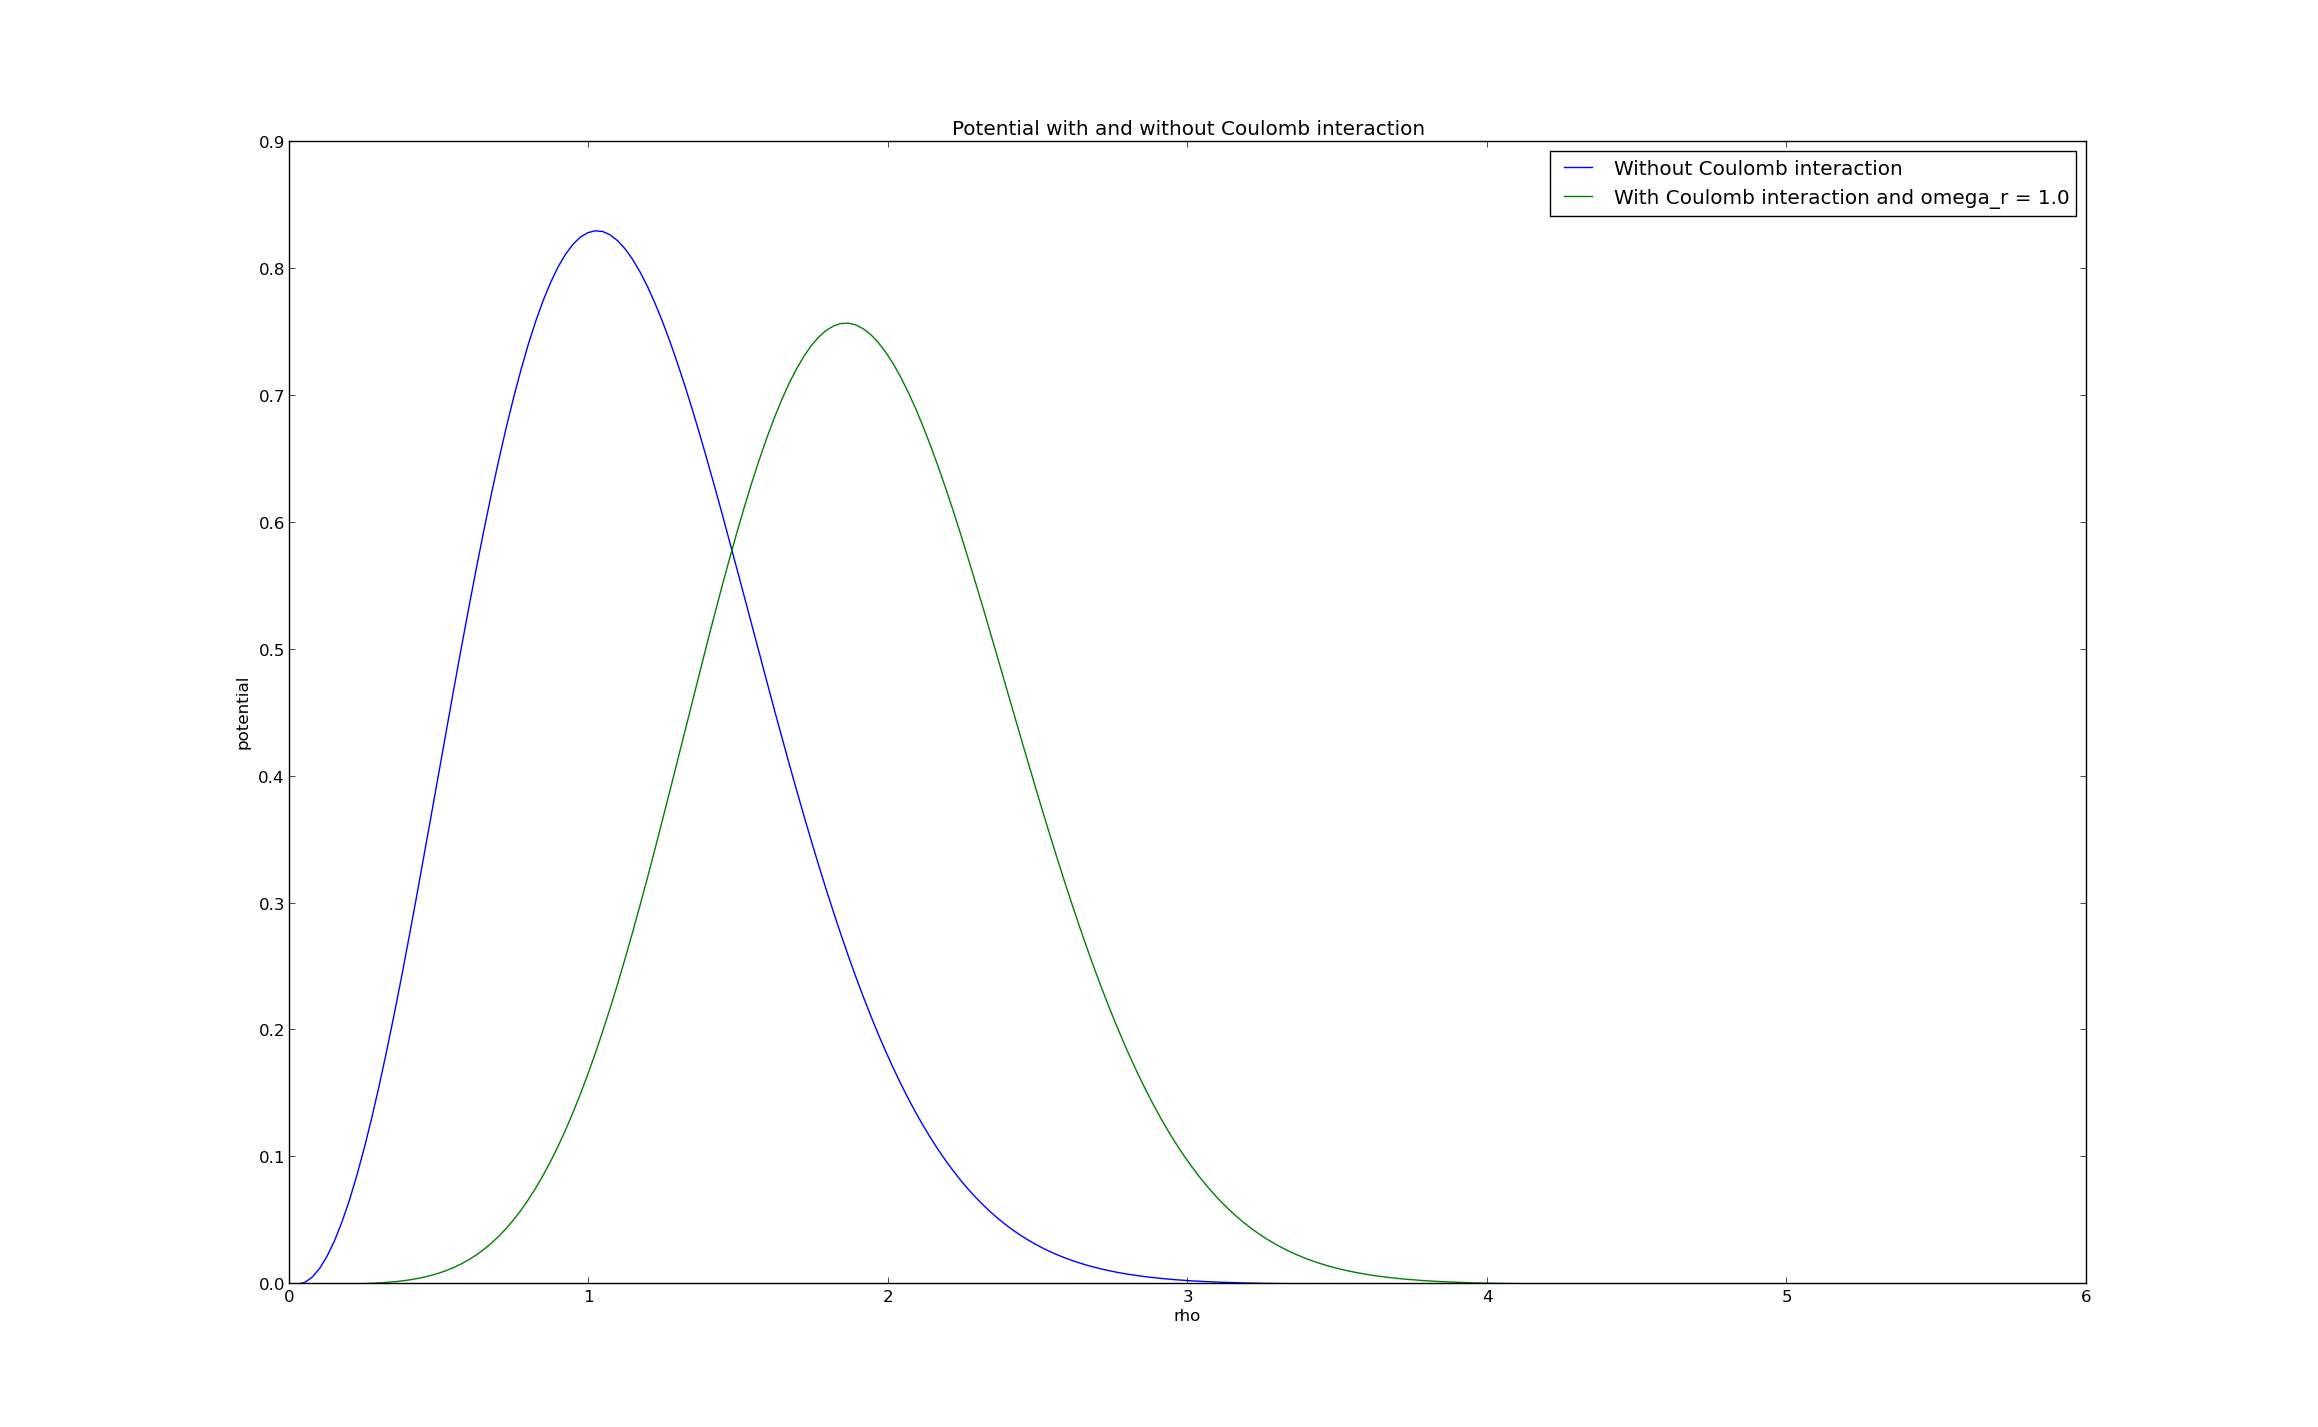
\includegraphics[width=400px]{omega1to10.png}
        \caption{Her er $V_i = \omega_r^2\rho^2 + \frac{10}{\rho}$ for den grøne grafen.}
      \end{figure}

    \subsubsection{Plott for $\omega_r = 5$}
      Den siste frekvensen vil gje oss ein bratt, men kort graf. Me får eit kraftig potensial for elektron i nærleiken av einannan. Her har me $\rho_{\text{max}} = 2$.
      \begin{figure}[H]
        \centering
        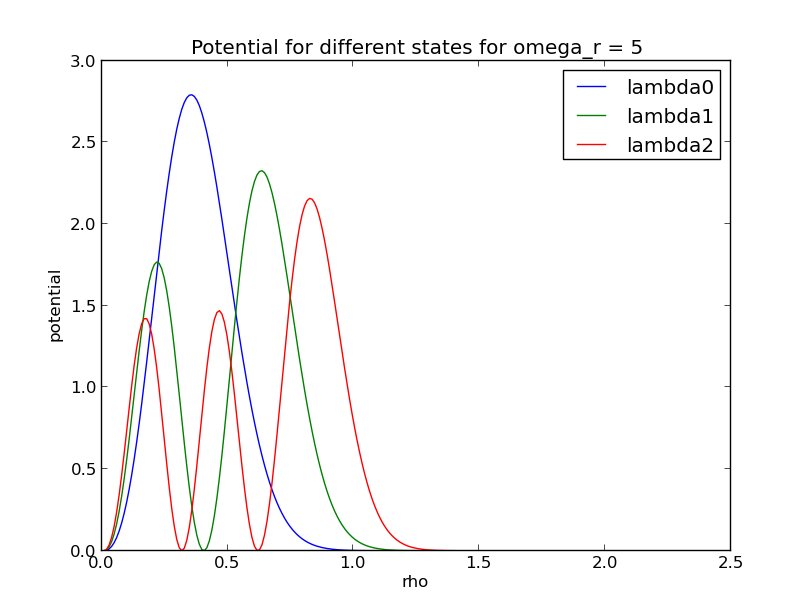
\includegraphics[width=300px]{omega5.png}
        \caption{Plott for $\rho_{\text{max}} = 2$ gjer oss ei kurve med eit stort potensial.}
      \end{figure}





    \subsubsection{Totalt}
      Under fylgjer eit plott over dei fire frekvensane i lag for å gje eit inntrykk over utviklinga.
      \begin{figure}[H]
        \centering
        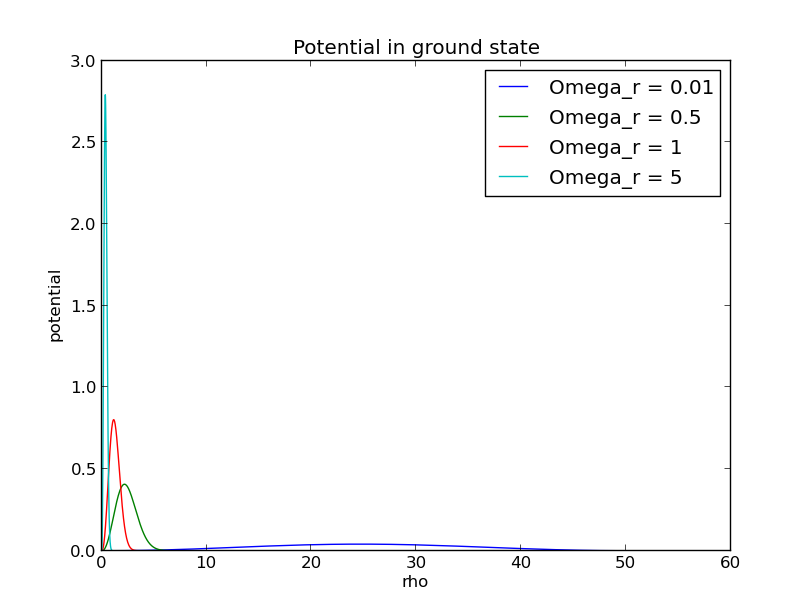
\includegraphics[width=300px]{total.png}
        \caption{Her er $\rho_{\text{max}}$ for $\omega_r = 0.01$ altfor låg, men viss me skrur opp verdien vil plottet bli veldig lite informativt.}
      \end{figure}

  \subsection{Feilanalyse}
    Eg har valt å inkludere ei lita feilanalyse for å få eit overblikk over kor lang tid det tek før Jacobis metode gjer oss fire siffers nøyaktighet (merk at det er her snakk om 
    siffer og ikkje desimal) på dei tre fyrste eigenverdiane. Diverre er ikkje dette eit enkelt svar då det avhenger av valet vårt av $\rho_{\text{max}}$. Eg har her 
    plotta $\log_{10}$ av differansen mellom den eksakte og den numeriske løsyninga (og trukket frå ein då $\log_{10}$ vil gje oss antal desimalar) mot $n_{step}$.
    
    \subsubsection{Plott for $\rho_{\text{max}} = 2$}
      \begin{figure}[H]
        \centering
        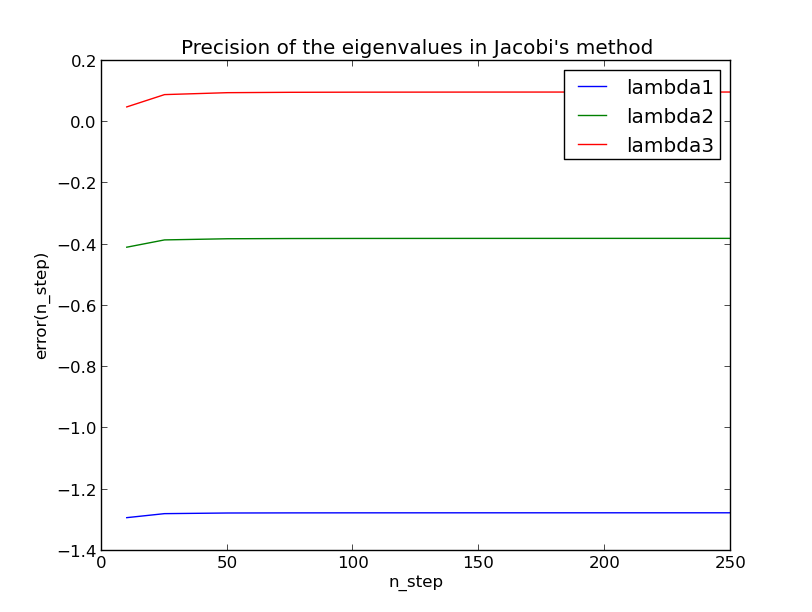
\includegraphics[width=300px]{feil2.png}
        \caption{Uttrykket me jobber med for potensialet er berekna for store verdiar av $\rho_{\text{max}}$. Me får difor store feil for dei eksakte eigenverdiane.}
      \end{figure}

    \subsubsection{Plott for $\rho_{\text{max}} = 3$}
      \begin{figure}[H]
        \centering
        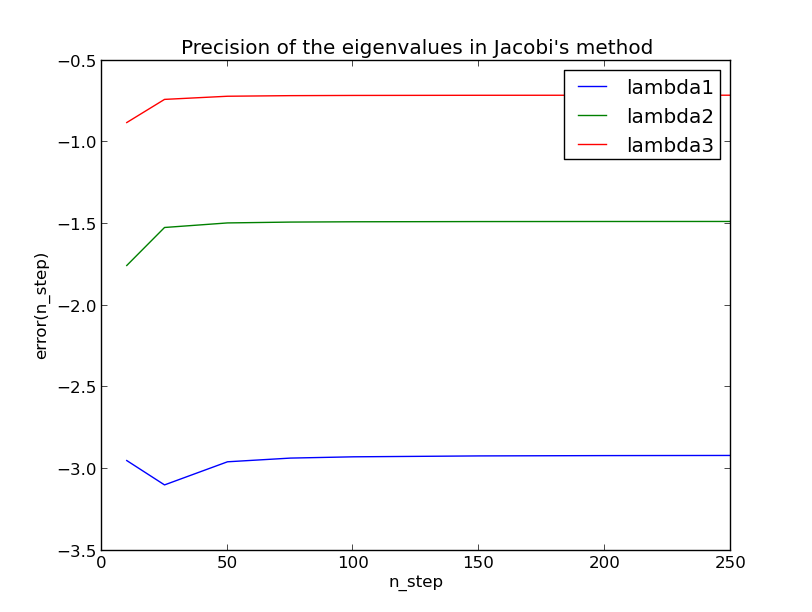
\includegraphics[width=300px]{feil3.png}
        \caption{Her har me mykje den same problematikken. Metoden vil sikte seg inn mot feil eigenverdi.}
      \end{figure}

    \subsubsection{Plott for $\rho_{\text{max}} = 4$}
      \begin{figure}[H]
        \centering
        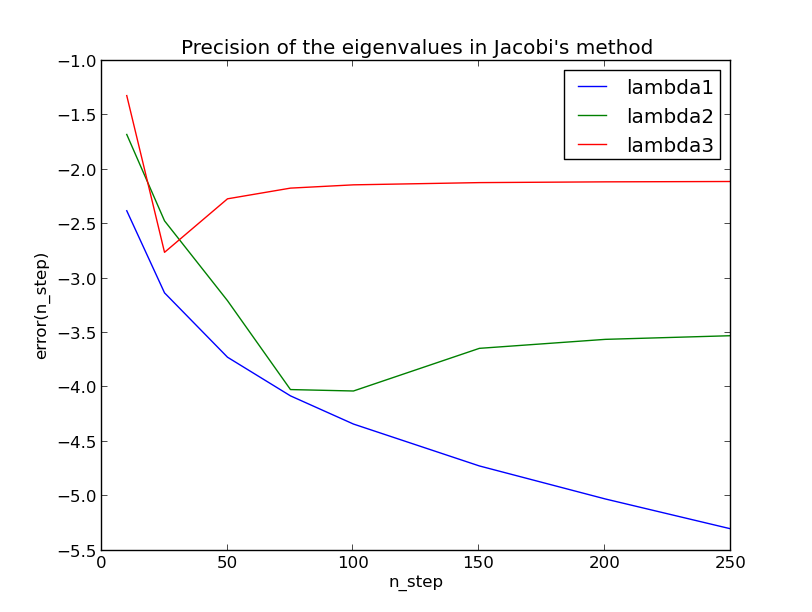
\includegraphics[width=300px]{feil4.png}
        \caption{Her byrjar metoden å fungere som han skal.}
      \end{figure}

    \subsubsection{Plott for $\rho_{\text{max}} = 5$}
      \begin{figure}[H]
        \centering
        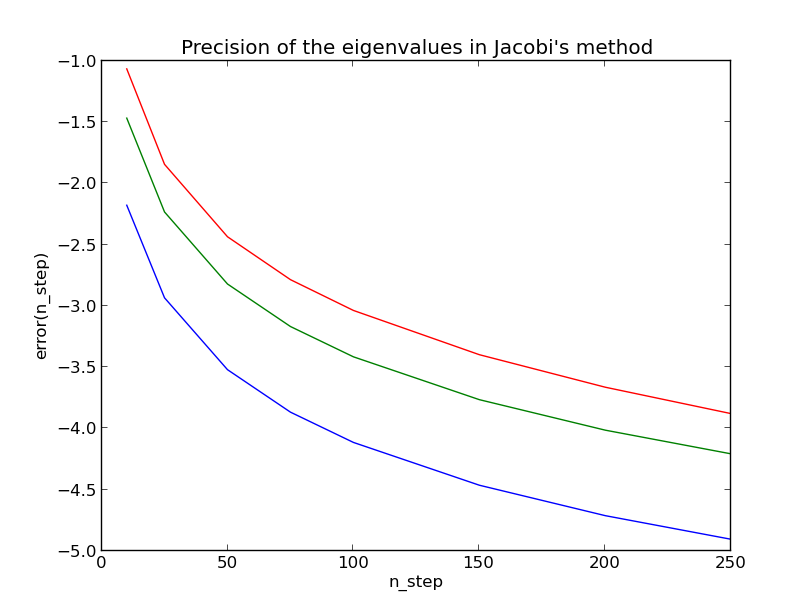
\includegraphics[width=300px]{feil5.png}
        \caption{For $\rho_{\text{max}} = 5$ får me oppførselen me vil ha.}
      \end{figure}

    \subsubsection{Plott for $\rho_{\text{max}} = 7$}
      \begin{figure}[H]
        \centering
        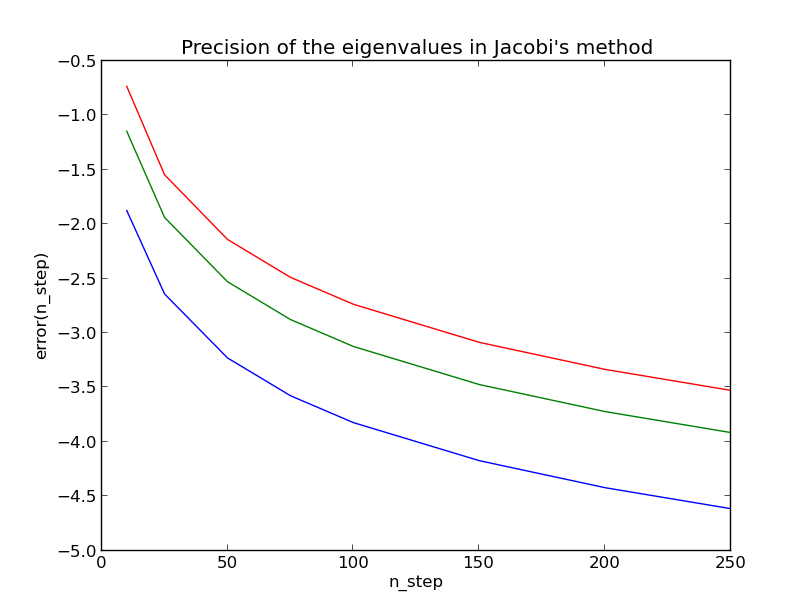
\includegraphics[width=300px]{feil7.png}
        \caption{Her kan me sjå korleis feilen byrjar å stige igjen.}
      \end{figure}

    \subsubsection{Plott for $\rho_{\text{max}} = 10$}
      \begin{figure}[H]
        \centering
        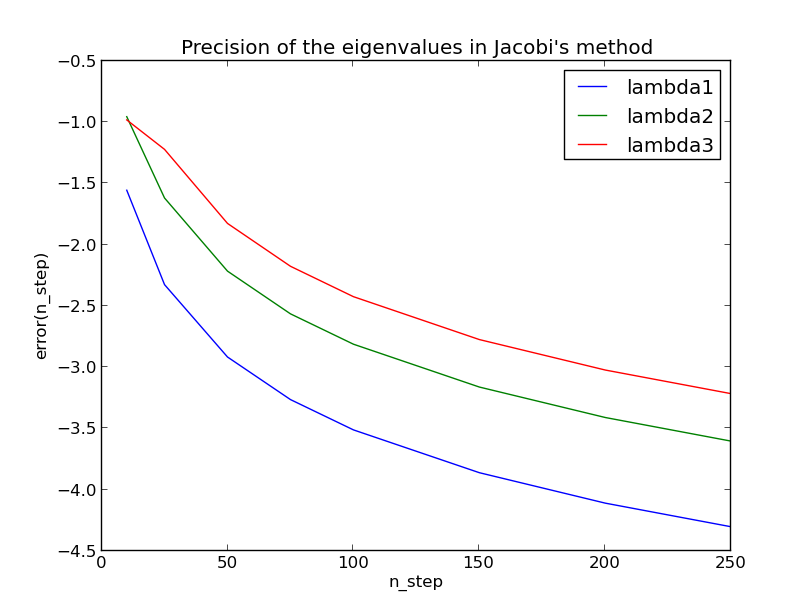
\includegraphics[width=300px]{feil10.png}
        \caption{Gradvis stig feilen igjen.}
      \end{figure}

    For $\rho_{\text{max}} = 5$ får me dei verdiane me ynskjer. For den fyrste eigenverdien klarer me nesten å få fem siffers nøyaktighet. Viss me minkar eller aukar 
    $\rho_{\text{max}}$ vil feilen stige igjen.

\end{document}
